\documentclass{article}

\usepackage{graphicx}
\usepackage{tikz}
\usepackage{tikzsymbols}
\usetikzlibrary{calc,patterns,shapes.geometric}
\pagestyle{empty}
\usepackage[margin=0pt]{geometry}
\geometry{papersize={14in,12in}}

\def\centerarc[#1](#2)(#3:#4:#5){\draw[#1] ($(#2)+({#5*cos(#3)},{#5*sin(#3)})$) arc (#3:#4:#5);}

\begin{document}
	\begin{figure}
		\centering
		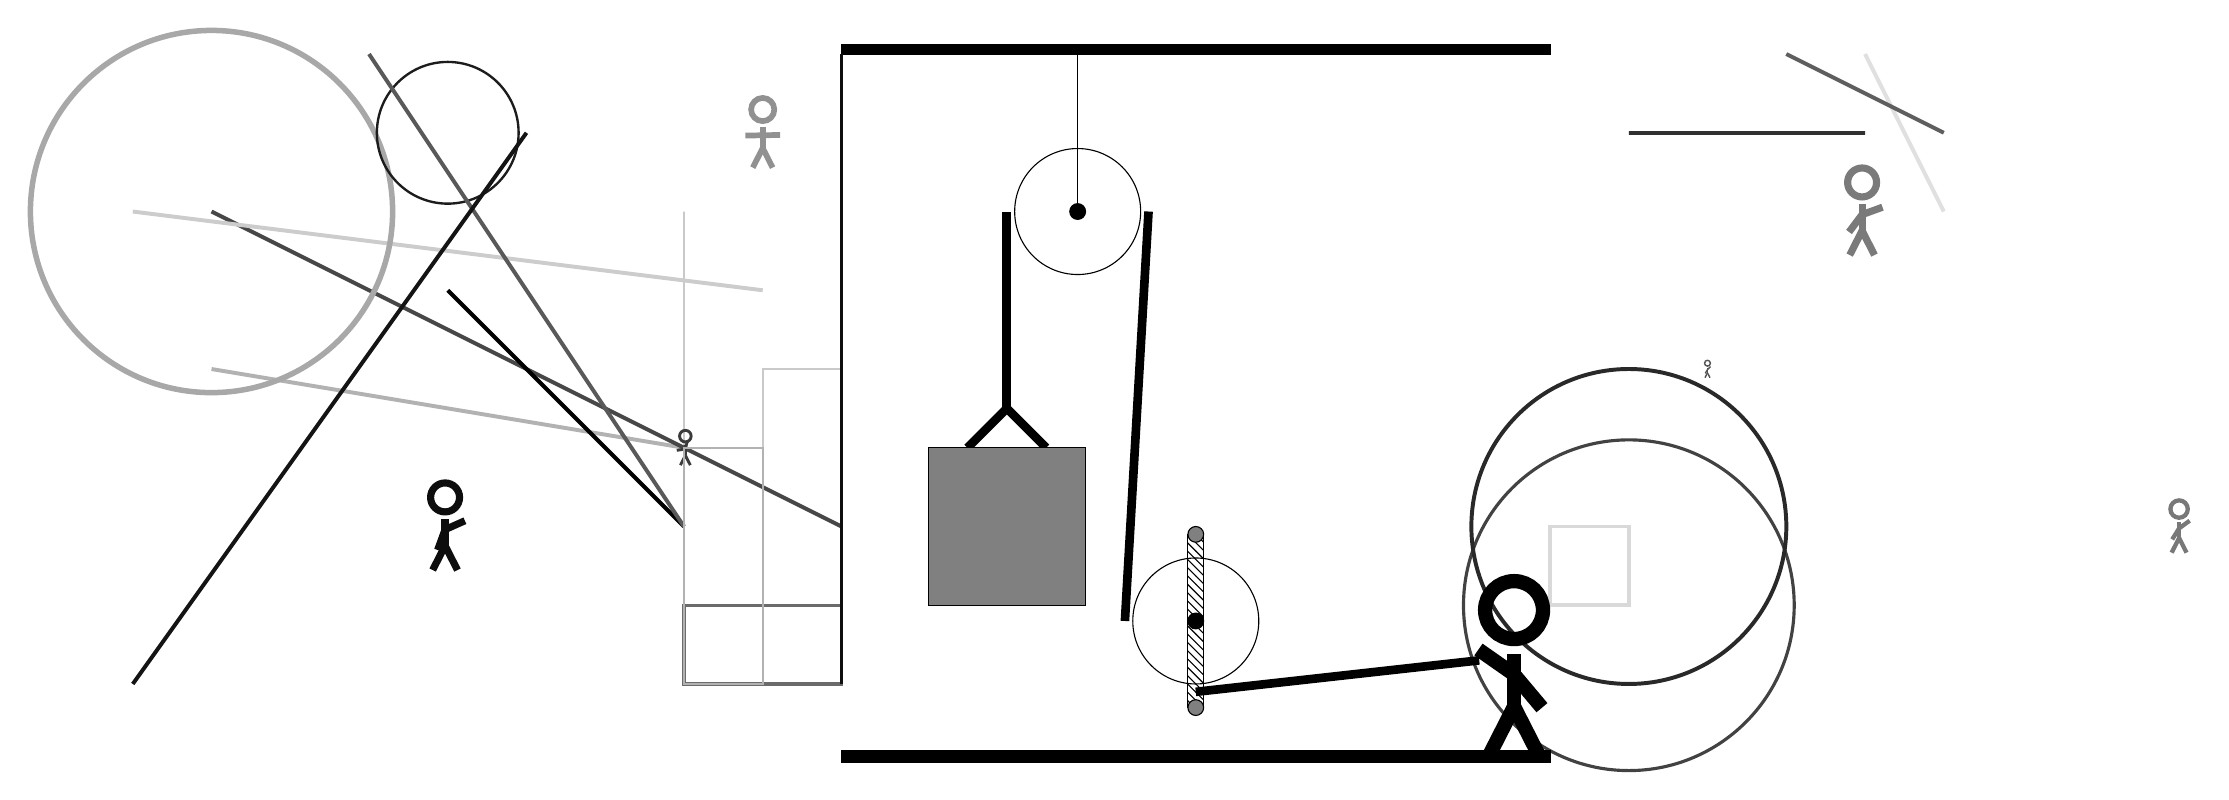
\begin{tikzpicture}
			%%%%% START %%%%%
			
			\draw[fill=black] (-2, 9) rectangle (7, 9.125);
			
			\draw (1, 7) circle (0.8);
			\draw[fill=black] (1, 7) circle (0.1);
			\draw (1, 9) -- (1, 7);
			
			\draw[fill=white](2.5, 1.8) circle (0.8);
			\draw[fill=black] (2.5, 1.8) circle (0.1);
			\draw[pattern=north west lines, pattern color=black] (2.4, 2.9) rectangle (2.6, 0.7);
			\draw[fill=black!50] (2.5, 2.9) circle (0.1);
			\draw[fill=black!50] (2.5, 0.7) circle (0.1);
			
			\draw [line width=0.4mm, color=black!74](8, 2) circle (2.1);
			
			\draw[line width=0.5mm, color=black!30](-4, 4) -- (-10, 5);
			\draw[line width=0.2mm, color=black!21] (-4, 1) rectangle (-4, 7);
			\draw[line width=0.5mm, color=black!81] (8, 8) rectangle (11, 8);
			
			\draw[line width=0.5mm, color=black!72](-2, 3) -- (-10, 7);
			\node[line width=0.3mm, color=black!95] at (-7, 3) {\Strichmaxerl[5][70][24]};
			\draw[line width=0.5mm, color=black!100](-4, 3) -- (-7, 6);
			
			\draw[line width=0.5mm, color=black!20](-3, 6) -- (-11, 7);
			\draw[line width=0.5mm, color=black!12](12, 7) -- (11, 9);
			\node[line width=0.6mm, color=black!52] at (11, 7) {\Strichmaxerl[5][53][20]};
			\node[line width=0.7mm, color=black!43] at (-3, 8) {\Strichmaxerl[4][1][1]};
			\node[line width=0.2mm, color=black!53] at (15, 3) {\Strichmaxerl[3][58][36]};
			\draw[line width=0.3mm, color=black!21] (-3, 1) rectangle (-2, 5);
			
			\draw[line width=0.5mm, color=black!15] (7, 2) rectangle (8, 3);
			\draw [line width=0.7mm, color=black!34](-10, 7) circle (2.3);
			\draw[line width=0.5mm, color=black!63](12, 8) -- (10, 9);
			
			\draw [line width=0.3mm, color=black!89](-7, 8) circle (0.9);
			
			\draw[line width=0.4mm, color=black!58] (-2, 2) rectangle (-4, 1);
			\draw [line width=0.5mm, color=black!84](8, 3) circle (2.0);
			\node[line width=0.3mm, color=black!67] at (9, 5) {\Strichmaxerl[1][59][44]};
			\draw[line width=0.5mm, color=black!65](-4, 3) -- (-8, 9);
			
			\draw[line width=0.5mm, color=black!92](-6, 8) -- (-11, 1);
			\draw[line width=0.4mm, color=black!94] (-2, 9) rectangle (-2, 1);
			\node[line width=0.7mm, color=black!77] at (-4, 4) {\Strichmaxerl[2][9][76]};
			\draw[line width=0.3mm, color=black!30] (-4, 4) rectangle (-3, 1);
			
			
			\draw[line width=1.1mm] (-0.4, 4.0) -- (0.1, 4.5) -- (0.6, 4.0);
			\draw[fill=black!50] (-0.9, 4.0) rectangle (1.1, 2.0);
			
			\draw[line width=1.1mm] (0.1, 7) -- (0.1, 4.5);
			\centerarc[line width=1.1mm](1, 7)(0:180:0.9);
			\draw[line width=1.1mm](1.9, 7) -- (1.6, 1.8);
			\centerarc[line width=1.1mm](2.5, 1.8)(180:270:0.9);
			\draw[line width=1.1mm](2.5, 0.9) -- (6.1, 1.3);
			
			\node at (6.5, 1.2) {\Strichmaxerl[10][-35][-50]};
			
			\draw[fill=black] (-2, 0) rectangle (7, 0.15);
			
			%%%%% END %%%%%
		\end{tikzpicture}
	\end{figure}	
\end{document}